\documentclass{article}
\usepackage{iclr2026_conference,times}
\usepackage{graphicx,booktabs,hyperref}
\iclrfinalcopy
\author{Local baseline project\\AI-assisted draft; not peer reviewed}
\title{Context Selection for Configuration History: A Reproducible JiuwenSwarm Pilot}
\begin{document}
\maketitle
\fancyhead[L]{Local baseline draft -- not submitted}
\begin{abstract}
This local synthetic pilot examines how different history-selection policies affect a single model's ability to answer questions about configuration state while controlling API token use. Using 24 deterministic synthetic histories of 60 records each, we compare four policies: full history, a recent-window baseline, lexical retrieval, and retrieval augmented with summaries. The full-history reference is unbounded, and selection budgets use a cl100k\_base tokenizer proxy, while measured resource totals use API-reported input and output tokens. All policies run in isolated sessions with the same model and temperature-zero decoding. Observed exact accuracy is 24/24 for full, retrieve, and retrieve\_summary, and 6/24 for recent. Paired comparisons show recent is correct only on late-position cases, while retrieve and retrieve\_summary match full on every case. Summary costs are included in token accounting. These results are descriptive for a synthetic convenience sample; Wilson intervals are not guarantees, and no equivalence or generalization claim is made. The pilot suggests that lexical retrieval can preserve configuration state at lower API token use than full history in this setting, but broader evaluation is required before any research claim.
\end{abstract}
\section{Introduction}
Agents that operate over long interaction histories face a practical tension: retaining enough context to answer questions about earlier configuration state while limiting the number of tokens sent to the model. Prior work has documented sensitivity to the position of relevant information in long contexts (Liu et al., 2023), and virtual context management has been proposed to manage memory across sessions (Packer et al., 2023). This pilot asks a narrow question: in a controlled synthetic setting, which history policy preserves configuration state while reducing API token use? We compare full history, a recent-window baseline, lexical retrieval, and retrieval with summaries. The full-history condition serves as an unbounded reference, not a deployable budget. The recent-window baseline tests whether recency alone suffices. Retrieval selects records by exact project-identifier matching, and retrieve\_summary adds a summary of the retrieved records. All policies use the same model and isolated sessions, and summary overhead is included in token accounting. The goal is not to introduce a new method or to claim benchmark validation, but to establish a cautious baseline for a reusable experiment pipeline.
\section{Related Work}
Liu et al. (2023) evaluate multi-document question answering and key-value retrieval and report sensitivity to the position of relevant information, motivating our early, middle, and late placement groups. Packer et al. (2023) introduce virtual context management inspired by hierarchical memory and evaluate document analysis and multi-session chat, which is conceptually related to our retrieval and summary policies. Yao et al. (2022) interleave reasoning and actions in language models; our pilot uses the ReActAgent class but disables tools and does not evaluate action planning. These references frame the problem space but do not provide the specific synthetic tasks or policies tested here. We make no novelty claim and do not assert that our retrieval approach is equivalent to prior systems. The pilot is a local synthetic study, not a held-out benchmark evaluation.
\section{Methods}
We constructed 24 deterministic synthetic histories with a fixed seed, each comprising 60 records. Tasks are grouped into three families: lookup, partial, and revision, with 8 tasks per family. Records are placed in early, middle, or late positions, yielding 9 early, 9 middle, and 6 late cases. Histories include field-wise overwrites to simulate configuration changes. Four policies are compared: full, recent, retrieve, and retrieve\_summary. Full sends the entire unbounded history. Recent sends only the most recent records within a proxy budget of 512 tokens. Retrieve selects records by exact project-identifier matching, also within the 512-token proxy budget. Retrieve\_summary summarizes the retrieved records within a 256-token proxy budget. Selection budgets use the cl100k\_base tokenizer as a proxy; measured resource totals are API-reported input and output tokens, including summary calls. All policies run with deepseek-flash through the official DeepSeek API, temperature 0, top\_p 1, thinking disabled, and isolated sessions. The agent processes a supplied static history in a single answering call; these are not observed multi-turn interactions. History selection is applied in before\_invoke, and actual calls are captured in after\_model\_call. Summary costs are included in token accounting. Scoring is exact match and field accuracy. Paired comparisons use exact McNemar tests, reported as exploratory and not corrected for multiple comparisons. Wilson intervals are descriptive only and are not guarantees.
\section{Measured Results}
Table~1 reports the saved paired run. Confidence intervals are descriptive Wilson intervals on a synthetic convenience sample. They do not establish generalization or equivalence.
All 120 experiment API calls succeeded, using 101768 API-reported tokens. Draft-writing and smoke-test usage are separately logged and excluded from the experiment table.
\begin{table}[ht]\centering\small
\begin{tabular}{lrrrrr}\toprule
Method & Correct & Acc. (\%) & 95\% CI & Tokens/task & Sec./task \\ \midrule
Full history & 24/24 & 100.0 & [86.2, 100.0] & 3111.0 & 0.71 \\
Recent window & 6/24 & 25.0 & [12.0, 44.9] & 636.8 & 0.72 \\
Project retrieval & 24/24 & 100.0 & [86.2, 100.0] & 175.5 & 0.68 \\
Retrieval + summary & 24/24 & 100.0 & [86.2, 100.0] & 317.0 & 1.43 \\
\bottomrule\end{tabular}
\caption{Measured results. Tokens include input, output, and summary overhead. Full history is an unbounded reference.}\end{table}
\begin{figure}[ht]\centering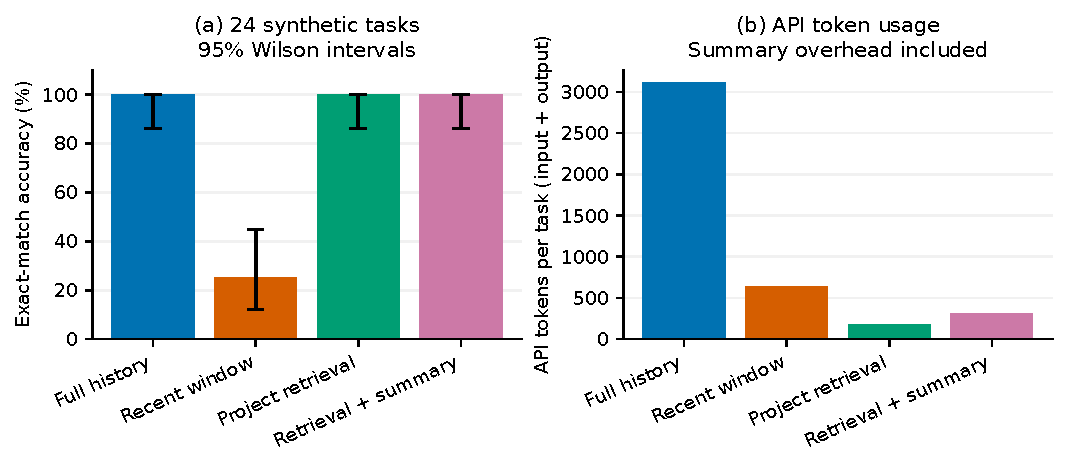
\includegraphics[width=\linewidth]{results_figure.pdf}
\caption{Exact-match accuracy with descriptive Wilson intervals, and API tokens per task.}\end{figure}
\section{Discussion}
The recent-window baseline fails on early and middle positions, consistent with omitted evidence rather than a general failure of recency. It is correct only on late-position cases, where the needed records fall within the recent window. Retrieve and retrieve\_summary match full on every case in this synthetic sample, but this should not be read as equivalence. The tasks favor lexical matching because questions and records share identifiers, which may overstate retrieval performance relative to more paraphrased or ambiguous settings. Adding summaries does not improve accuracy over retrieval alone here, and it increases API calls and mean seconds per task, though total API-reported tokens remain lower than full. The full-history reference is unbounded, so token comparisons are descriptive rather than budget-matched. Wilson intervals are wide and descriptive; they are not guarantees. The paired McNemar results are exploratory and uncorrected. This is a local synthetic pilot, not benchmark validation, and it does not establish real-world agent performance or long-context robustness. No novelty or equivalence claim is made.
\section{Conclusion}
In this local synthetic pilot, lexical retrieval and retrieval with summaries preserved configuration state as well as an unbounded full-history reference on 24 tasks, while a recent-window baseline succeeded only on late-position cases. Summary overhead is included in token accounting, and all policies used the same model in isolated sessions. These findings are descriptive for a synthetic convenience sample; Wilson intervals are not guarantees, and paired tests are exploratory. The pilot contributes a reusable opt-in JiuwenSwarm rail and a verified experiment pipeline, but broader evaluation with held-out benchmarks, varied tokenizers, and real multi-turn interactions is required before any research claim. We do not claim equivalence, novelty, or generalization.
\section{Generation and Reproducibility Disclosure}
Codex assisted with question selection, code, dataset generation, execution, and draft review. DeepSeek produced compressed contexts and the initial manuscript prose from the saved evidence bundle. Measured tables are inserted programmatically. No independent human review or Stanford Agentic Reviewer assessment has been performed. The new rail is loaded directly from the JiuwenSwarm source checkout and registered on openJiuwen ReActAgent; the full JiuwenSwarm GUI/Swarm assembly is not part of this experiment. Source patch, generator, logs, and reproduction commands accompany this draft.
\begin{thebibliography}{9}
\bibitem[Liu et al.(2023)]{liu2023} Nelson F. Liu, Kevin Lin, John Hewitt, Ashwin Paranjape, Michele Bevilacqua, Fabio Petroni, and Percy Liang. Lost in the Middle: How Language Models Use Long Contexts. 2023. \url{https://arxiv.org/abs/2307.03172}.
\bibitem[Packer et al.(2023)]{packer2023} Charles Packer, Sarah Wooders, Kevin Lin, Vivian Fang, Shishir G. Patil, Ion Stoica, and Joseph E. Gonzalez. MemGPT: Towards LLMs as Operating Systems. 2023. \url{https://arxiv.org/abs/2310.08560}.
\bibitem[Yao et al.(2022)]{yao2022} Shunyu Yao, Jeffrey Zhao, Dian Yu, Nan Du, Izhak Shafran, Karthik Narasimhan, and Yuan Cao. ReAct: Synergizing Reasoning and Acting in Language Models. 2022. \url{https://arxiv.org/abs/2210.03629}.
\end{thebibliography}
\end{document}